\customHeader{1}{\finetuning{}}
\label{06_finetuning}

Finetuning, in the context of \gls{nlp}, refers to the process of taking a pre-trained language model and further training it on a specific task or dataset. At the outset, we use a pre-trained model, which has undergone training on a vast dataset, enabling it to grasp general features and patterns applicable to a broad spectrum of tasks. \finetuning{} allows us to adapt the pre-trained model to a more specific domain by updating its parameters using task-specific data.


In our scenario, \gls{bert} embeddings are used for document classification. To tailor the model to our particular task, we enable the backpropagation process to adjust not only the classification layer but also the weights of the \gls{bert} model (refer to Figure \ref{fig:06_finetuning_bert_for_document_classification} in contrast to Figure \ref{fig:02_bert_for_document_classification}). This technique allows us to make the  \gls{bert} model adapt the way it produces embeddings and learn a representation of our documents which is more convenient for our task.

Given the imbalance in our datasets, we employ weighted cross-entropy as the loss. Yet, our initial experiments revealed that artificially balancing the dataset enhanced performance. Further details can be found in \headerName{} \ref{06_splitting_the_dataset}.


\begin{figure}
    \centering
    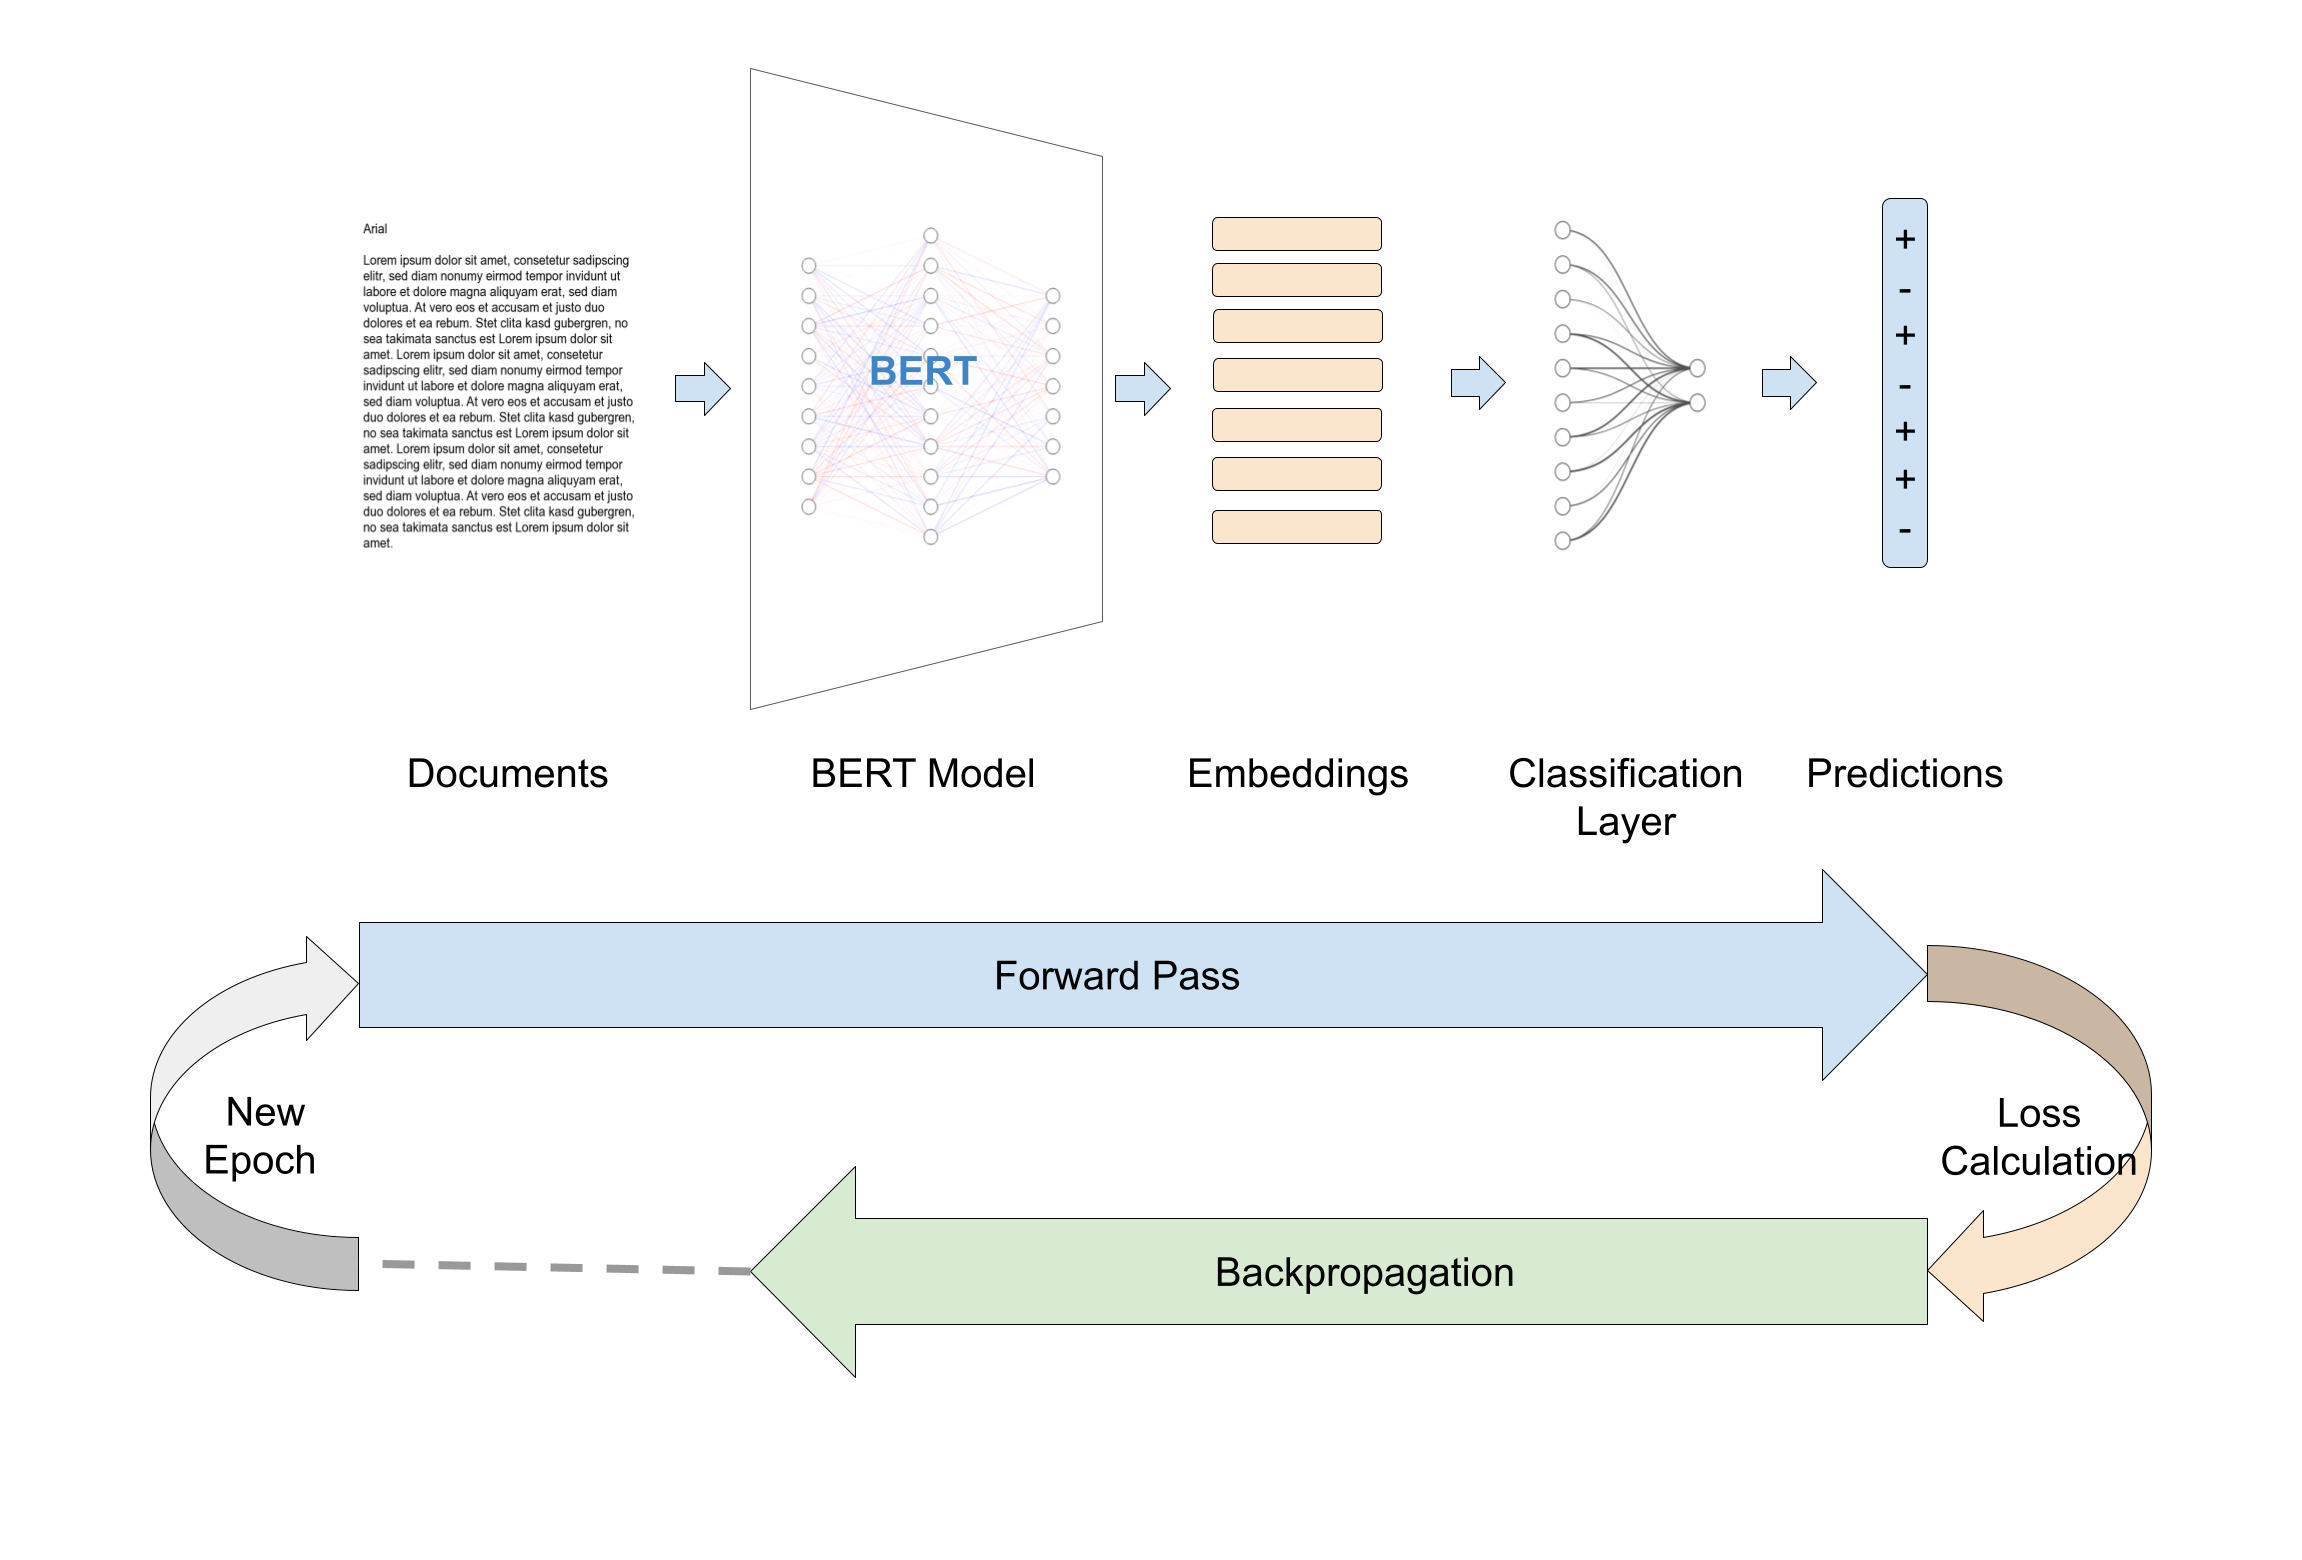
\includegraphics[width=\textwidth]{Figures/06/06_BERT_finetuning.png}
    \caption{\finetuning{} \BERT{} for Document Classification}
    \label{fig:06_finetuning_bert_for_document_classification}
\end{figure}
